\documentclass[1p]{elsarticle_modified}
%\bibliographystyle{elsarticle-num}

%\usepackage[colorlinks]{hyperref}
%\usepackage{abbrmath_seonhwa} %\Abb, \Ascr, \Acal ,\Abf, \Afrak
\usepackage{amsfonts}
\usepackage{amssymb}
\usepackage{amsmath}
\usepackage{amsthm}
\usepackage{scalefnt}
\usepackage{amsbsy}
\usepackage{kotex}
\usepackage{caption}
\usepackage{subfig}
\usepackage{color}
\usepackage{graphicx}
\usepackage{xcolor} %% white, black, red, green, blue, cyan, magenta, yellow
\usepackage{float}
\usepackage{setspace}
\usepackage{hyperref}

\usepackage{tikz}
\usetikzlibrary{arrows}

\usepackage{multirow}
\usepackage{array} % fixed length table
\usepackage{hhline}

%%%%%%%%%%%%%%%%%%%%%
\makeatletter
\renewcommand*\env@matrix[1][\arraystretch]{%
	\edef\arraystretch{#1}%
	\hskip -\arraycolsep
	\let\@ifnextchar\new@ifnextchar
	\array{*\c@MaxMatrixCols c}}
\makeatother %https://tex.stackexchange.com/questions/14071/how-can-i-increase-the-line-spacing-in-a-matrix
%%%%%%%%%%%%%%%

\usepackage[normalem]{ulem}

\newcommand{\msout}[1]{\ifmmode\text{\sout{\ensuremath{#1}}}\else\sout{#1}\fi}
%SOURCE: \msout is \stkout macro in https://tex.stackexchange.com/questions/20609/strikeout-in-math-mode

\newcommand{\cancel}[1]{
	\ifmmode
	{\color{red}\msout{#1}}
	\else
	{\color{red}\sout{#1}}
	\fi
}

\newcommand{\add}[1]{
	{\color{blue}\uwave{#1}}
}

\newcommand{\replace}[2]{
	\ifmmode
	{\color{red}\msout{#1}}{\color{blue}\uwave{#2}}
	\else
	{\color{red}\sout{#1}}{\color{blue}\uwave{#2}}
	\fi
}

\newcommand{\Sol}{\mathcal{S}} %segment
\newcommand{\D}{D} %diagram
\newcommand{\A}{\mathcal{A}} %arc


%%%%%%%%%%%%%%%%%%%%%%%%%%%%%5 test

\def\sl{\operatorname{\textup{SL}}(2,\Cbb)}
\def\psl{\operatorname{\textup{PSL}}(2,\Cbb)}
\def\quan{\mkern 1mu \triangleright \mkern 1mu}

\theoremstyle{definition}
\newtheorem{thm}{Theorem}[section]
\newtheorem{prop}[thm]{Proposition}
\newtheorem{lem}[thm]{Lemma}
\newtheorem{ques}[thm]{Question}
\newtheorem{cor}[thm]{Corollary}
\newtheorem{defn}[thm]{Definition}
\newtheorem{exam}[thm]{Example}
\newtheorem{rmk}[thm]{Remark}
\newtheorem{alg}[thm]{Algorithm}

\newcommand{\I}{\sqrt{-1}}
\begin{document}

%\begin{frontmatter}
%
%\title{Boundary parabolic representations of knots up to 8 crossings}
%
%%% Group authors per affiliation:
%\author{Yunhi Cho} 
%\address{Department of Mathematics, University of Seoul, Seoul, Korea}
%\ead{yhcho@uos.ac.kr}
%
%
%\author{Seonhwa Kim} %\fnref{s_kim}}
%\address{Center for Geometry and Physics, Institute for Basic Science, Pohang, 37673, Korea}
%\ead{ryeona17@ibs.re.kr}
%
%\author{Hyuk Kim}
%\address{Department of Mathematical Sciences, Seoul National University, Seoul 08826, Korea}
%\ead{hyukkim@snu.ac.kr}
%
%\author{Seokbeom Yoon}
%\address{Department of Mathematical Sciences, Seoul National University, Seoul, 08826,  Korea}
%\ead{sbyoon15@snu.ac.kr}
%
%\begin{abstract}
%We find all boundary parabolic representation of knots up to 8 crossings.
%
%\end{abstract}
%\begin{keyword}
%    \MSC[2010] 57M25 
%\end{keyword}
%
%\end{frontmatter}

%\linenumbers
%\tableofcontents
%
\newcommand\colored[1]{\textcolor{white}{\rule[-0.35ex]{0.8em}{1.4ex}}\kern-0.8em\color{red} #1}%
%\newcommand\colored[1]{\textcolor{white}{ #1}\kern-2.17ex	\textcolor{white}{ #1}\kern-1.81ex	\textcolor{white}{ #1}\kern-2.15ex\color{red}#1	}

{\Large $\underline{12a_{0366}~(K12a_{0366})}$}

\setlength{\tabcolsep}{10pt}
\renewcommand{\arraystretch}{1.6}
\vspace{1cm}\begin{tabular}{m{100pt}>{\centering\arraybackslash}m{274pt}}
\multirow{5}{120pt}{
	\centering
	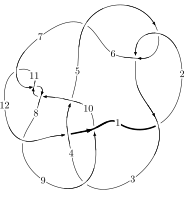
\includegraphics[width=112pt]{../../../GIT/diagram.site/Diagrams/png/1167_12a_0366.png}\\
\ \ \ A knot diagram\footnotemark}&
\allowdisplaybreaks
\textbf{Linearized knot diagam} \\
\cline{2-2}
 &
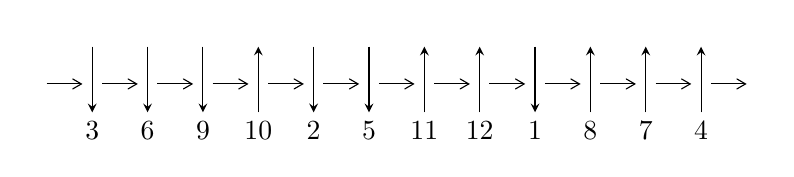
\begin{tikzpicture}[x=20pt, y=17pt]
	% nodes
	\node (C0) at (0, 0) {};
	\node (C1) at (1, 0) {};
	\node (C1U) at (1, +1) {};
	\node (C1D) at (1, -1) {3};

	\node (C2) at (2, 0) {};
	\node (C2U) at (2, +1) {};
	\node (C2D) at (2, -1) {6};

	\node (C3) at (3, 0) {};
	\node (C3U) at (3, +1) {};
	\node (C3D) at (3, -1) {9};

	\node (C4) at (4, 0) {};
	\node (C4U) at (4, +1) {};
	\node (C4D) at (4, -1) {10};

	\node (C5) at (5, 0) {};
	\node (C5U) at (5, +1) {};
	\node (C5D) at (5, -1) {2};

	\node (C6) at (6, 0) {};
	\node (C6U) at (6, +1) {};
	\node (C6D) at (6, -1) {5};

	\node (C7) at (7, 0) {};
	\node (C7U) at (7, +1) {};
	\node (C7D) at (7, -1) {11};

	\node (C8) at (8, 0) {};
	\node (C8U) at (8, +1) {};
	\node (C8D) at (8, -1) {12};

	\node (C9) at (9, 0) {};
	\node (C9U) at (9, +1) {};
	\node (C9D) at (9, -1) {1};

	\node (C10) at (10, 0) {};
	\node (C10U) at (10, +1) {};
	\node (C10D) at (10, -1) {8};

	\node (C11) at (11, 0) {};
	\node (C11U) at (11, +1) {};
	\node (C11D) at (11, -1) {7};

	\node (C12) at (12, 0) {};
	\node (C12U) at (12, +1) {};
	\node (C12D) at (12, -1) {4};
	\node (C13) at (13, 0) {};

	% arrows
	\draw[->,>={angle 60}]
	(C0) edge (C1) (C1) edge (C2) (C2) edge (C3) (C3) edge (C4) (C4) edge (C5) (C5) edge (C6) (C6) edge (C7) (C7) edge (C8) (C8) edge (C9) (C9) edge (C10) (C10) edge (C11) (C11) edge (C12) (C12) edge (C13) ;	\draw[->,>=stealth]
	(C1U) edge (C1D) (C2U) edge (C2D) (C3U) edge (C3D) (C4D) edge (C4U) (C5U) edge (C5D) (C6U) edge (C6D) (C7D) edge (C7U) (C8D) edge (C8U) (C9U) edge (C9D) (C10D) edge (C10U) (C11D) edge (C11U) (C12D) edge (C12U) ;
	\end{tikzpicture} \\
\hhline{~~} \\& 
\textbf{Solving Sequence} \\ \cline{2-2} 
 &
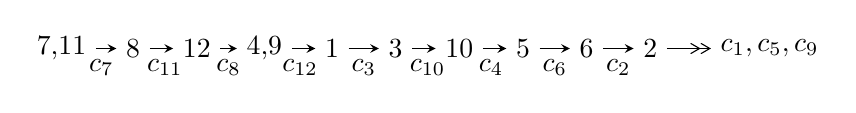
\begin{tikzpicture}[x=23pt, y=7pt]
	% node
	\node (A0) at (-1/8, 0) {7,11};
	\node (A1) at (1, 0) {8};
	\node (A2) at (2, 0) {12};
	\node (A3) at (49/16, 0) {4,9};
	\node (A4) at (33/8, 0) {1};
	\node (A5) at (41/8, 0) {3};
	\node (A6) at (49/8, 0) {10};
	\node (A7) at (57/8, 0) {5};
	\node (A8) at (65/8, 0) {6};
	\node (A9) at (73/8, 0) {2};
	\node (C1) at (1/2, -1) {$c_{7}$};
	\node (C2) at (3/2, -1) {$c_{11}$};
	\node (C3) at (5/2, -1) {$c_{8}$};
	\node (C4) at (29/8, -1) {$c_{12}$};
	\node (C5) at (37/8, -1) {$c_{3}$};
	\node (C6) at (45/8, -1) {$c_{10}$};
	\node (C7) at (53/8, -1) {$c_{4}$};
	\node (C8) at (61/8, -1) {$c_{6}$};
	\node (C9) at (69/8, -1) {$c_{2}$};
	\node (A10) at (11, 0) {$c_{1},c_{5},c_{9}$};

	% edge
	\draw[->,>=stealth]	
	(A0) edge (A1) (A1) edge (A2) (A2) edge (A3) (A3) edge (A4) (A4) edge (A5) (A5) edge (A6) (A6) edge (A7) (A7) edge (A8) (A8) edge (A9) ;
	\draw[->>,>={angle 60}]	
	(A9) edge (A10);
\end{tikzpicture} \\ 

\end{tabular} \\

\footnotetext{
The image of knot diagram is generated by the software ``\textbf{Draw programme}" developed by Andrew Bartholomew(\url{http://www.layer8.co.uk/maths/draw/index.htm\#Running-draw}), where we modified some parts for our purpose(\url{https://github.com/CATsTAILs/LinksPainter}).
}\phantom \\ \newline 
\centering \textbf{Ideals for irreducible components\footnotemark of $X_{\text{par}}$} 
 
\begin{align*}
I^u_{1}&=\langle 
-1.20161\times10^{100} u^{98}-1.07370\times10^{101} u^{97}+\cdots+5.32115\times10^{101} b-4.79500\times10^{101},\\
\phantom{I^u_{1}}&\phantom{= \langle  }4.08591\times10^{101} u^{98}-9.54872\times10^{101} u^{97}+\cdots+5.32115\times10^{101} a+2.76802\times10^{102},\;u^{99}-2 u^{98}+\cdots+10 u-1\rangle \\
I^u_{2}&=\langle 
b- u+1,\;- u^2+a-2 u-1,\;u^3+u^2+2 u+1\rangle \\
\\
\end{align*}
\raggedright * 2 irreducible components of $\dim_{\mathbb{C}}=0$, with total 102 representations.\\
\footnotetext{All coefficients of polynomials are rational numbers. But the coefficients are sometimes approximated in decimal forms when there is not enough margin.}
\newpage
\renewcommand{\arraystretch}{1}
\centering \section*{I. $I^u_{1}= \langle -1.20\times10^{100} u^{98}-1.07\times10^{101} u^{97}+\cdots+5.32\times10^{101} b-4.80\times10^{101},\;4.09\times10^{101} u^{98}-9.55\times10^{101} u^{97}+\cdots+5.32\times10^{101} a+2.77\times10^{102},\;u^{99}-2 u^{98}+\cdots+10 u-1 \rangle$}
\flushleft \textbf{(i) Arc colorings}\\
\begin{tabular}{m{7pt} m{180pt} m{7pt} m{180pt} }
\flushright $a_{7}=$&$\begin{pmatrix}1\\0\end{pmatrix}$ \\
\flushright $a_{11}=$&$\begin{pmatrix}0\\u\end{pmatrix}$ \\
\flushright $a_{8}=$&$\begin{pmatrix}1\\- u^2\end{pmatrix}$ \\
\flushright $a_{12}=$&$\begin{pmatrix}u\\u\end{pmatrix}$ \\
\flushright $a_{4}=$&$\begin{pmatrix}-0.767862 u^{98}+1.79449 u^{97}+\cdots-12.3985 u-5.20192\\0.0225817 u^{98}+0.201779 u^{97}+\cdots-1.34732 u+0.901122\end{pmatrix}$ \\
\flushright $a_{9}=$&$\begin{pmatrix}- u^4- u^2+1\\- u^4-2 u^2\end{pmatrix}$ \\
\flushright $a_{1}=$&$\begin{pmatrix}0.861849 u^{98}-1.09544 u^{97}+\cdots+2.79010 u+3.49312\\0.0199269 u^{98}+0.608326 u^{97}+\cdots+4.08418 u-0.841922\end{pmatrix}$ \\
\flushright $a_{3}=$&$\begin{pmatrix}-0.725424 u^{98}+1.49057 u^{97}+\cdots-16.5479 u-4.17999\\0.00155011 u^{98}+0.0452744 u^{97}+\cdots-2.59505 u+0.978516\end{pmatrix}$ \\
\flushright $a_{10}=$&$\begin{pmatrix}- u\\u^3+u\end{pmatrix}$ \\
\flushright $a_{5}=$&$\begin{pmatrix}-0.725766 u^{98}+1.41165 u^{97}+\cdots-14.9928 u-4.96501\\0.00320677 u^{98}-0.0365230 u^{97}+\cdots-1.78152 u+0.962855\end{pmatrix}$ \\
\flushright $a_{6}=$&$\begin{pmatrix}0.854628 u^{98}-1.62697 u^{97}+\cdots-5.36906 u+6.43646\\0.0502721 u^{98}+0.0347137 u^{97}+\cdots+0.693556 u-0.831628\end{pmatrix}$ \\
\flushright $a_{2}=$&$\begin{pmatrix}-0.0293994 u^{98}+0.0890561 u^{97}+\cdots+8.63836 u-1.36250\\-0.0197781 u^{98}+0.0447446 u^{97}+\cdots+2.48760 u+0.0270043\end{pmatrix}$\\&\end{tabular}
\flushleft \textbf{(ii) Obstruction class $= -1$}\\~\\
\flushleft \textbf{(iii) Cusp Shapes $= -0.817358 u^{98}+1.60477 u^{97}+\cdots+11.3028 u-8.84250$}\\~\\
\newpage\renewcommand{\arraystretch}{1}
\flushleft \textbf{(iv) u-Polynomials at the component}\newline \\
\begin{tabular}{m{50pt}|m{274pt}}
Crossings & \hspace{64pt}u-Polynomials at each crossing \\
\hline $$\begin{aligned}c_{1},c_{6}\end{aligned}$$&$\begin{aligned}
&u^{99}+30 u^{98}+\cdots+11 u+1
\end{aligned}$\\
\hline $$\begin{aligned}c_{2},c_{5}\end{aligned}$$&$\begin{aligned}
&u^{99}+4 u^{98}+\cdots-3 u+1
\end{aligned}$\\
\hline $$\begin{aligned}c_{3}\end{aligned}$$&$\begin{aligned}
&u^{99}-2 u^{98}+\cdots-30950 u+10543
\end{aligned}$\\
\hline $$\begin{aligned}c_{4}\end{aligned}$$&$\begin{aligned}
&u^{99}+38 u^{97}+\cdots+2168454 u+308593
\end{aligned}$\\
\hline $$\begin{aligned}c_{7},c_{10},c_{11}\end{aligned}$$&$\begin{aligned}
&u^{99}+2 u^{98}+\cdots+10 u+1
\end{aligned}$\\
\hline $$\begin{aligned}c_{8}\end{aligned}$$&$\begin{aligned}
&u^{99}-2 u^{98}+\cdots+20112 u+7633
\end{aligned}$\\
\hline $$\begin{aligned}c_{9}\end{aligned}$$&$\begin{aligned}
&u^{99}+7 u^{98}+\cdots-4 u-8
\end{aligned}$\\
\hline $$\begin{aligned}c_{12}\end{aligned}$$&$\begin{aligned}
&u^{99}+10 u^{98}+\cdots- u+1
\end{aligned}$\\
\hline
\end{tabular}\\~\\
\newpage\renewcommand{\arraystretch}{1}
\flushleft \textbf{(v) Riley Polynomials at the component}\newline \\
\begin{tabular}{m{50pt}|m{274pt}}
Crossings & \hspace{64pt}Riley Polynomials at each crossing \\
\hline $$\begin{aligned}c_{1},c_{6}\end{aligned}$$&$\begin{aligned}
&y^{99}+82 y^{98}+\cdots+267 y-1
\end{aligned}$\\
\hline $$\begin{aligned}c_{2},c_{5}\end{aligned}$$&$\begin{aligned}
&y^{99}-30 y^{98}+\cdots+11 y-1
\end{aligned}$\\
\hline $$\begin{aligned}c_{3}\end{aligned}$$&$\begin{aligned}
&y^{99}+132 y^{98}+\cdots-3285085678 y-111154849
\end{aligned}$\\
\hline $$\begin{aligned}c_{4}\end{aligned}$$&$\begin{aligned}
&y^{99}+76 y^{98}+\cdots+5233821340866 y-95229639649
\end{aligned}$\\
\hline $$\begin{aligned}c_{7},c_{10},c_{11}\end{aligned}$$&$\begin{aligned}
&y^{99}+84 y^{98}+\cdots+146 y-1
\end{aligned}$\\
\hline $$\begin{aligned}c_{8}\end{aligned}$$&$\begin{aligned}
&y^{99}-44 y^{98}+\cdots+8103212674 y-58262689
\end{aligned}$\\
\hline $$\begin{aligned}c_{9}\end{aligned}$$&$\begin{aligned}
&y^{99}+21 y^{98}+\cdots-1968 y-64
\end{aligned}$\\
\hline $$\begin{aligned}c_{12}\end{aligned}$$&$\begin{aligned}
&y^{99}-10 y^{98}+\cdots+11 y-1
\end{aligned}$\\
\hline
\end{tabular}\\~\\
\newpage\flushleft \textbf{(vi) Complex Volumes and Cusp Shapes}
$$\begin{array}{c|c|c}  
\text{Solutions to }I^u_{1}& \I (\text{vol} + \sqrt{-1}CS) & \text{Cusp shape}\\
 \hline 
\begin{aligned}
u &= -0.934041 + 0.285611 I \\
a &= \phantom{-}0.0684546 - 0.1098530 I \\
b &= \phantom{-}0.760126 - 0.032980 I\end{aligned}
 & \phantom{-}6.44395 - 4.31125 I & \phantom{-0.000000 } 0 \\ \hline\begin{aligned}
u &= -0.934041 - 0.285611 I \\
a &= \phantom{-}0.0684546 + 0.1098530 I \\
b &= \phantom{-}0.760126 + 0.032980 I\end{aligned}
 & \phantom{-}6.44395 + 4.31125 I & \phantom{-0.000000 } 0 \\ \hline\begin{aligned}
u &= -0.945397 + 0.242380 I \\
a &= -0.0894131 + 0.0864711 I \\
b &= -0.777045 + 0.023858 I\end{aligned}
 & \phantom{-}6.51992 + 1.59072 I & \phantom{-0.000000 } 0 \\ \hline\begin{aligned}
u &= -0.945397 - 0.242380 I \\
a &= -0.0894131 - 0.0864711 I \\
b &= -0.777045 - 0.023858 I\end{aligned}
 & \phantom{-}6.51992 - 1.59072 I & \phantom{-0.000000 } 0 \\ \hline\begin{aligned}
u &= -0.619852 + 0.849329 I \\
a &= -0.191895 - 0.725655 I \\
b &= \phantom{-}0.451994 - 0.354754 I\end{aligned}
 & \phantom{-}4.65474 - 1.02924 I & \phantom{-0.000000 } 0 \\ \hline\begin{aligned}
u &= -0.619852 - 0.849329 I \\
a &= -0.191895 + 0.725655 I \\
b &= \phantom{-}0.451994 + 0.354754 I\end{aligned}
 & \phantom{-}4.65474 + 1.02924 I & \phantom{-0.000000 } 0 \\ \hline\begin{aligned}
u &= \phantom{-}0.489624 + 0.976166 I \\
a &= \phantom{-}1.11011 + 1.17258 I \\
b &= \phantom{-}0.862929 - 0.009132 I\end{aligned}
 & \phantom{-}5.00008 - 8.91845 I & \phantom{-0.000000 } 0 \\ \hline\begin{aligned}
u &= \phantom{-}0.489624 - 0.976166 I \\
a &= \phantom{-}1.11011 - 1.17258 I \\
b &= \phantom{-}0.862929 + 0.009132 I\end{aligned}
 & \phantom{-}5.00008 + 8.91845 I & \phantom{-0.000000 } 0 \\ \hline\begin{aligned}
u &= -0.607360 + 0.910741 I \\
a &= \phantom{-}0.158283 + 0.794060 I \\
b &= -0.453491 + 0.410887 I\end{aligned}
 & \phantom{-}4.43226 - 6.94743 I & \phantom{-0.000000 } 0 \\ \hline\begin{aligned}
u &= -0.607360 - 0.910741 I \\
a &= \phantom{-}0.158283 - 0.794060 I \\
b &= -0.453491 - 0.410887 I\end{aligned}
 & \phantom{-}4.43226 + 6.94743 I & \phantom{-0.000000 } 0\\
 \hline 
 \end{array}$$\newpage$$\begin{array}{c|c|c}  
\text{Solutions to }I^u_{1}& \I (\text{vol} + \sqrt{-1}CS) & \text{Cusp shape}\\
 \hline 
\begin{aligned}
u &= \phantom{-}0.465505 + 1.006420 I \\
a &= -1.13331 - 1.17177 I \\
b &= -0.868308 - 0.003082 I\end{aligned}
 & \phantom{-}5.66290 - 2.75362 I & \phantom{-0.000000 } 0 \\ \hline\begin{aligned}
u &= \phantom{-}0.465505 - 1.006420 I \\
a &= -1.13331 + 1.17177 I \\
b &= -0.868308 + 0.003082 I\end{aligned}
 & \phantom{-}5.66290 + 2.75362 I & \phantom{-0.000000 } 0 \\ \hline\begin{aligned}
u &= -0.295504 + 1.081280 I \\
a &= \phantom{-}0.274270 + 1.370950 I \\
b &= -0.157652 + 0.819914 I\end{aligned}
 & -1.54134 - 4.00958 I & \phantom{-0.000000 } 0 \\ \hline\begin{aligned}
u &= -0.295504 - 1.081280 I \\
a &= \phantom{-}0.274270 - 1.370950 I \\
b &= -0.157652 - 0.819914 I\end{aligned}
 & -1.54134 + 4.00958 I & \phantom{-0.000000 } 0 \\ \hline\begin{aligned}
u &= \phantom{-}0.848820 + 0.223053 I \\
a &= \phantom{-}0.1302910 - 0.0495279 I \\
b &= \phantom{-}1.63335 + 0.71600 I\end{aligned}
 & \phantom{-}7.3252 + 13.6606 I & \phantom{-0.000000 } 0. - 8.92570 I \\ \hline\begin{aligned}
u &= \phantom{-}0.848820 - 0.223053 I \\
a &= \phantom{-}0.1302910 + 0.0495279 I \\
b &= \phantom{-}1.63335 - 0.71600 I\end{aligned}
 & \phantom{-}7.3252 - 13.6606 I & \phantom{-0.000000 -}0. + 8.92570 I \\ \hline\begin{aligned}
u &= \phantom{-}0.307610 + 0.818157 I \\
a &= \phantom{-}1.08566 + 1.28137 I \\
b &= \phantom{-}0.697402 + 0.013200 I\end{aligned}
 & -1.99276 - 4.20196 I & \phantom{-0.000000 } 0 \\ \hline\begin{aligned}
u &= \phantom{-}0.307610 - 0.818157 I \\
a &= \phantom{-}1.08566 - 1.28137 I \\
b &= \phantom{-}0.697402 - 0.013200 I\end{aligned}
 & -1.99276 + 4.20196 I & \phantom{-0.000000 } 0 \\ \hline\begin{aligned}
u &= \phantom{-}0.844705 + 0.201410 I \\
a &= -0.113791 + 0.098540 I \\
b &= -1.62516 - 0.71635 I\end{aligned}
 & \phantom{-}8.14139 + 7.42066 I & \phantom{-}5.24860 - 4.23174 I \\ \hline\begin{aligned}
u &= \phantom{-}0.844705 - 0.201410 I \\
a &= -0.113791 - 0.098540 I \\
b &= -1.62516 + 0.71635 I\end{aligned}
 & \phantom{-}8.14139 - 7.42066 I & \phantom{-}5.24860 + 4.23174 I\\
 \hline 
 \end{array}$$\newpage$$\begin{array}{c|c|c}  
\text{Solutions to }I^u_{1}& \I (\text{vol} + \sqrt{-1}CS) & \text{Cusp shape}\\
 \hline 
\begin{aligned}
u &= \phantom{-}0.248263 + 1.118570 I \\
a &= -1.32465 - 1.35187 I \\
b &= -1.028980 - 0.184164 I\end{aligned}
 & \phantom{-}0.608522 - 0.603280 I & \phantom{-0.000000 } 0 \\ \hline\begin{aligned}
u &= \phantom{-}0.248263 - 1.118570 I \\
a &= -1.32465 + 1.35187 I \\
b &= -1.028980 + 0.184164 I\end{aligned}
 & \phantom{-}0.608522 + 0.603280 I & \phantom{-0.000000 } 0 \\ \hline\begin{aligned}
u &= \phantom{-}0.752592 + 0.215634 I \\
a &= -0.1157960 - 0.0197121 I \\
b &= \phantom{-}1.63356 + 0.74026 I\end{aligned}
 & \phantom{-}0.05606 + 8.13743 I & -0.09558 - 8.89965 I \\ \hline\begin{aligned}
u &= \phantom{-}0.752592 - 0.215634 I \\
a &= -0.1157960 + 0.0197121 I \\
b &= \phantom{-}1.63356 - 0.74026 I\end{aligned}
 & \phantom{-}0.05606 - 8.13743 I & -0.09558 + 8.89965 I \\ \hline\begin{aligned}
u &= \phantom{-}0.268779 + 1.199880 I \\
a &= \phantom{-}0.24849 + 1.92674 I \\
b &= \phantom{-}1.48419 + 1.59594 I\end{aligned}
 & \phantom{-}3.35814 - 2.05345 I & \phantom{-0.000000 } 0 \\ \hline\begin{aligned}
u &= \phantom{-}0.268779 - 1.199880 I \\
a &= \phantom{-}0.24849 - 1.92674 I \\
b &= \phantom{-}1.48419 - 1.59594 I\end{aligned}
 & \phantom{-}3.35814 + 2.05345 I & \phantom{-0.000000 } 0 \\ \hline\begin{aligned}
u &= \phantom{-}0.745362 + 0.134461 I \\
a &= \phantom{-}0.175401 + 0.260812 I \\
b &= -1.61882 - 0.76689 I\end{aligned}
 & \phantom{-}3.52295 + 4.31748 I & \phantom{-}6.92910 - 5.56695 I \\ \hline\begin{aligned}
u &= \phantom{-}0.745362 - 0.134461 I \\
a &= \phantom{-}0.175401 - 0.260812 I \\
b &= -1.61882 + 0.76689 I\end{aligned}
 & \phantom{-}3.52295 - 4.31748 I & \phantom{-}6.92910 + 5.56695 I \\ \hline\begin{aligned}
u &= -0.678642 + 0.330251 I \\
a &= -0.206249 - 0.013125 I \\
b &= \phantom{-}0.615264 + 0.077383 I\end{aligned}
 & \phantom{-}1.02146 - 1.90927 I & \phantom{-}5.91964 + 9.92466 I \\ \hline\begin{aligned}
u &= -0.678642 - 0.330251 I \\
a &= -0.206249 + 0.013125 I \\
b &= \phantom{-}0.615264 - 0.077383 I\end{aligned}
 & \phantom{-}1.02146 + 1.90927 I & \phantom{-}5.91964 - 9.92466 I\\
 \hline 
 \end{array}$$\newpage$$\begin{array}{c|c|c}  
\text{Solutions to }I^u_{1}& \I (\text{vol} + \sqrt{-1}CS) & \text{Cusp shape}\\
 \hline 
\begin{aligned}
u &= -0.754120\phantom{ +0.000000I} \\
a &= -0.187188\phantom{ +0.000000I} \\
b &= -0.890755\phantom{ +0.000000I}\end{aligned}
 & \phantom{-}1.70898\phantom{ +0.000000I} & \phantom{-}8.74420\phantom{ +0.000000I} \\ \hline\begin{aligned}
u &= -0.029724 + 1.250120 I \\
a &= \phantom{-}0.98004 + 2.06746 I \\
b &= \phantom{-}0.97006 + 1.27890 I\end{aligned}
 & -1.32263 - 4.42952 I & \phantom{-0.000000 } 0 \\ \hline\begin{aligned}
u &= -0.029724 - 1.250120 I \\
a &= \phantom{-}0.98004 - 2.06746 I \\
b &= \phantom{-}0.97006 - 1.27890 I\end{aligned}
 & -1.32263 + 4.42952 I & \phantom{-0.000000 } 0 \\ \hline\begin{aligned}
u &= \phantom{-}0.745953 + 0.036112 I \\
a &= \phantom{-}0.006297 - 0.821786 I \\
b &= -1.42040 + 0.84753 I\end{aligned}
 & \phantom{-}7.64308 - 0.65029 I & \phantom{-}9.33071 + 0.18867 I \\ \hline\begin{aligned}
u &= \phantom{-}0.745953 - 0.036112 I \\
a &= \phantom{-}0.006297 + 0.821786 I \\
b &= -1.42040 - 0.84753 I\end{aligned}
 & \phantom{-}7.64308 + 0.65029 I & \phantom{-}9.33071 - 0.18867 I \\ \hline\begin{aligned}
u &= \phantom{-}0.732406 + 0.078855 I \\
a &= \phantom{-}0.062991 + 0.954918 I \\
b &= \phantom{-}1.33124 - 0.85513 I\end{aligned}
 & \phantom{-}6.74172 + 5.69863 I & \phantom{-}7.43474 - 6.11480 I \\ \hline\begin{aligned}
u &= \phantom{-}0.732406 - 0.078855 I \\
a &= \phantom{-}0.062991 - 0.954918 I \\
b &= \phantom{-}1.33124 + 0.85513 I\end{aligned}
 & \phantom{-}6.74172 - 5.69863 I & \phantom{-}7.43474 + 6.11480 I \\ \hline\begin{aligned}
u &= -0.734635\phantom{ +0.000000I} \\
a &= -0.210505\phantom{ +0.000000I} \\
b &= -0.911518\phantom{ +0.000000I}\end{aligned}
 & \phantom{-}1.70946\phantom{ +0.000000I} & \phantom{-}7.92140\phantom{ +0.000000I} \\ \hline\begin{aligned}
u &= \phantom{-}0.295125 + 1.232170 I \\
a &= -0.35967 - 2.03807 I \\
b &= -1.59104 - 1.63787 I\end{aligned}
 & \phantom{-}3.97750 + 4.41856 I & \phantom{-0.000000 } 0 \\ \hline\begin{aligned}
u &= \phantom{-}0.295125 - 1.232170 I \\
a &= -0.35967 + 2.03807 I \\
b &= -1.59104 + 1.63787 I\end{aligned}
 & \phantom{-}3.97750 - 4.41856 I & \phantom{-0.000000 } 0\\
 \hline 
 \end{array}$$\newpage$$\begin{array}{c|c|c}  
\text{Solutions to }I^u_{1}& \I (\text{vol} + \sqrt{-1}CS) & \text{Cusp shape}\\
 \hline 
\begin{aligned}
u &= \phantom{-}0.217724 + 1.257540 I \\
a &= \phantom{-}1.92175 + 1.50783 I \\
b &= \phantom{-}1.68088 + 0.04262 I\end{aligned}
 & -4.15077 + 2.23479 I & \phantom{-0.000000 } 0 \\ \hline\begin{aligned}
u &= \phantom{-}0.217724 - 1.257540 I \\
a &= \phantom{-}1.92175 - 1.50783 I \\
b &= \phantom{-}1.68088 - 0.04262 I\end{aligned}
 & -4.15077 - 2.23479 I & \phantom{-0.000000 } 0 \\ \hline\begin{aligned}
u &= -0.119234 + 1.301930 I \\
a &= -0.82700 - 2.40146 I \\
b &= -0.86265 - 1.81488 I\end{aligned}
 & -1.130880 + 0.549874 I & \phantom{-0.000000 } 0 \\ \hline\begin{aligned}
u &= -0.119234 - 1.301930 I \\
a &= -0.82700 + 2.40146 I \\
b &= -0.86265 + 1.81488 I\end{aligned}
 & -1.130880 - 0.549874 I & \phantom{-0.000000 } 0 \\ \hline\begin{aligned}
u &= -0.252218 + 1.284100 I \\
a &= \phantom{-}1.73380 + 2.17731 I \\
b &= \phantom{-}2.07810 + 1.91250 I\end{aligned}
 & \phantom{-}0.531022 - 0.352290 I & \phantom{-0.000000 } 0 \\ \hline\begin{aligned}
u &= -0.252218 - 1.284100 I \\
a &= \phantom{-}1.73380 - 2.17731 I \\
b &= \phantom{-}2.07810 - 1.91250 I\end{aligned}
 & \phantom{-}0.531022 + 0.352290 I & \phantom{-0.000000 } 0 \\ \hline\begin{aligned}
u &= \phantom{-}0.312678 + 1.284840 I \\
a &= -1.56503 - 0.86630 I \\
b &= -1.052390 + 0.317344 I\end{aligned}
 & \phantom{-}3.53108 + 3.17609 I & \phantom{-0.000000 } 0 \\ \hline\begin{aligned}
u &= \phantom{-}0.312678 - 1.284840 I \\
a &= -1.56503 + 0.86630 I \\
b &= -1.052390 - 0.317344 I\end{aligned}
 & \phantom{-}3.53108 - 3.17609 I & \phantom{-0.000000 } 0 \\ \hline\begin{aligned}
u &= -0.254772 + 1.300720 I \\
a &= -1.73085 - 2.36656 I \\
b &= -2.04108 - 2.08187 I\end{aligned}
 & \phantom{-}0.37869 - 6.12549 I & \phantom{-0.000000 } 0 \\ \hline\begin{aligned}
u &= -0.254772 - 1.300720 I \\
a &= -1.73085 + 2.36656 I \\
b &= -2.04108 + 2.08187 I\end{aligned}
 & \phantom{-}0.37869 + 6.12549 I & \phantom{-0.000000 } 0\\
 \hline 
 \end{array}$$\newpage$$\begin{array}{c|c|c}  
\text{Solutions to }I^u_{1}& \I (\text{vol} + \sqrt{-1}CS) & \text{Cusp shape}\\
 \hline 
\begin{aligned}
u &= -0.175162 + 1.316190 I \\
a &= \phantom{-}1.62898 + 0.27564 I \\
b &= \phantom{-}2.07408 + 0.32600 I\end{aligned}
 & -4.07709 - 2.24905 I & \phantom{-0.000000 } 0 \\ \hline\begin{aligned}
u &= -0.175162 - 1.316190 I \\
a &= \phantom{-}1.62898 - 0.27564 I \\
b &= \phantom{-}2.07408 - 0.32600 I\end{aligned}
 & -4.07709 + 2.24905 I & \phantom{-0.000000 } 0 \\ \hline\begin{aligned}
u &= -0.210759 + 1.318290 I \\
a &= -1.31219 - 3.45789 I \\
b &= -1.41862 - 3.15690 I\end{aligned}
 & -4.33937 - 2.97560 I & \phantom{-0.000000 } 0 \\ \hline\begin{aligned}
u &= -0.210759 - 1.318290 I \\
a &= -1.31219 + 3.45789 I \\
b &= -1.41862 + 3.15690 I\end{aligned}
 & -4.33937 + 2.97560 I & \phantom{-0.000000 } 0 \\ \hline\begin{aligned}
u &= -0.279170 + 1.313540 I \\
a &= -0.72178 + 1.46138 I \\
b &= -1.05622 + 1.14287 I\end{aligned}
 & -2.50644 - 3.56316 I & \phantom{-0.000000 } 0 \\ \hline\begin{aligned}
u &= -0.279170 - 1.313540 I \\
a &= -0.72178 - 1.46138 I \\
b &= -1.05622 - 1.14287 I\end{aligned}
 & -2.50644 + 3.56316 I & \phantom{-0.000000 } 0 \\ \hline\begin{aligned}
u &= \phantom{-}0.012646 + 1.346570 I \\
a &= \phantom{-}0.111304 + 0.574163 I \\
b &= \phantom{-}0.910249 + 0.778259 I\end{aligned}
 & -5.09149 - 1.65450 I & \phantom{-0.000000 } 0 \\ \hline\begin{aligned}
u &= \phantom{-}0.012646 - 1.346570 I \\
a &= \phantom{-}0.111304 - 0.574163 I \\
b &= \phantom{-}0.910249 - 0.778259 I\end{aligned}
 & -5.09149 + 1.65450 I & \phantom{-0.000000 } 0 \\ \hline\begin{aligned}
u &= \phantom{-}0.306416 + 1.314380 I \\
a &= \phantom{-}1.56544 + 0.71108 I \\
b &= \phantom{-}0.975960 - 0.437826 I\end{aligned}
 & \phantom{-}2.37552 + 9.45911 I & \phantom{-0.000000 } 0 \\ \hline\begin{aligned}
u &= \phantom{-}0.306416 - 1.314380 I \\
a &= \phantom{-}1.56544 - 0.71108 I \\
b &= \phantom{-}0.975960 + 0.437826 I\end{aligned}
 & \phantom{-}2.37552 - 9.45911 I & \phantom{-0.000000 } 0\\
 \hline 
 \end{array}$$\newpage$$\begin{array}{c|c|c}  
\text{Solutions to }I^u_{1}& \I (\text{vol} + \sqrt{-1}CS) & \text{Cusp shape}\\
 \hline 
\begin{aligned}
u &= \phantom{-}0.639595 + 0.091648 I \\
a &= -0.632784 - 0.391435 I \\
b &= \phantom{-}1.74029 + 0.82376 I\end{aligned}
 & -0.579400 + 0.781243 I & \phantom{-}3.90058 - 9.11901 I \\ \hline\begin{aligned}
u &= \phantom{-}0.639595 - 0.091648 I \\
a &= -0.632784 + 0.391435 I \\
b &= \phantom{-}1.74029 - 0.82376 I\end{aligned}
 & -0.579400 - 0.781243 I & \phantom{-}3.90058 + 9.11901 I \\ \hline\begin{aligned}
u &= -0.643484 + 0.012521 I \\
a &= \phantom{-}0.00320 - 2.60568 I \\
b &= \phantom{-}0.01890 - 1.95574 I\end{aligned}
 & \phantom{-}4.51074 - 2.88147 I & -21.2227 - 0.3778 I \\ \hline\begin{aligned}
u &= -0.643484 - 0.012521 I \\
a &= \phantom{-}0.00320 + 2.60568 I \\
b &= \phantom{-}0.01890 + 1.95574 I\end{aligned}
 & \phantom{-}4.51074 + 2.88147 I & -21.2227 + 0.3778 I \\ \hline\begin{aligned}
u &= \phantom{-}0.267449 + 1.332400 I \\
a &= \phantom{-}0.76039 + 2.51755 I \\
b &= \phantom{-}1.93430 + 1.74894 I\end{aligned}
 & -5.08797 + 4.10505 I & \phantom{-0.000000 } 0 \\ \hline\begin{aligned}
u &= \phantom{-}0.267449 - 1.332400 I \\
a &= \phantom{-}0.76039 - 2.51755 I \\
b &= \phantom{-}1.93430 - 1.74894 I\end{aligned}
 & -5.08797 - 4.10505 I & \phantom{-0.000000 } 0 \\ \hline\begin{aligned}
u &= \phantom{-}0.100202 + 1.368080 I \\
a &= \phantom{-}0.422862 - 0.568821 I \\
b &= -0.508707 - 0.941569 I\end{aligned}
 & -7.19579 + 2.54584 I & \phantom{-0.000000 } 0 \\ \hline\begin{aligned}
u &= \phantom{-}0.100202 - 1.368080 I \\
a &= \phantom{-}0.422862 + 0.568821 I \\
b &= -0.508707 + 0.941569 I\end{aligned}
 & -7.19579 - 2.54584 I & \phantom{-0.000000 } 0 \\ \hline\begin{aligned}
u &= \phantom{-}0.313104 + 1.345580 I \\
a &= -0.80767 - 2.26450 I \\
b &= -1.86910 - 1.64443 I\end{aligned}
 & -1.14017 + 8.15162 I & \phantom{-0.000000 } 0 \\ \hline\begin{aligned}
u &= \phantom{-}0.313104 - 1.345580 I \\
a &= -0.80767 + 2.26450 I \\
b &= -1.86910 + 1.64443 I\end{aligned}
 & -1.14017 - 8.15162 I & \phantom{-0.000000 } 0\\
 \hline 
 \end{array}$$\newpage$$\begin{array}{c|c|c}  
\text{Solutions to }I^u_{1}& \I (\text{vol} + \sqrt{-1}CS) & \text{Cusp shape}\\
 \hline 
\begin{aligned}
u &= \phantom{-}0.31190 + 1.38433 I \\
a &= \phantom{-}0.94240 + 2.25156 I \\
b &= \phantom{-}1.90592 + 1.61257 I\end{aligned}
 & -5.01093 + 11.99980 I & \phantom{-0.000000 } 0 \\ \hline\begin{aligned}
u &= \phantom{-}0.31190 - 1.38433 I \\
a &= \phantom{-}0.94240 - 2.25156 I \\
b &= \phantom{-}1.90592 - 1.61257 I\end{aligned}
 & -5.01093 - 11.99980 I & \phantom{-0.000000 } 0 \\ \hline\begin{aligned}
u &= \phantom{-}0.35666 + 1.39025 I \\
a &= -0.94316 - 2.12935 I \\
b &= -1.89156 - 1.57991 I\end{aligned}
 & \phantom{-}3.10562 + 11.74730 I & \phantom{-0.000000 } 0 \\ \hline\begin{aligned}
u &= \phantom{-}0.35666 - 1.39025 I \\
a &= -0.94316 + 2.12935 I \\
b &= -1.89156 + 1.57991 I\end{aligned}
 & \phantom{-}3.10562 - 11.74730 I & \phantom{-0.000000 } 0 \\ \hline\begin{aligned}
u &= -0.29273 + 1.41546 I \\
a &= \phantom{-}0.598510 - 0.901346 I \\
b &= \phantom{-}1.022280 - 0.601144 I\end{aligned}
 & -4.51107 - 5.52495 I & \phantom{-0.000000 } 0 \\ \hline\begin{aligned}
u &= -0.29273 - 1.41546 I \\
a &= \phantom{-}0.598510 + 0.901346 I \\
b &= \phantom{-}1.022280 + 0.601144 I\end{aligned}
 & -4.51107 + 5.52495 I & \phantom{-0.000000 } 0 \\ \hline\begin{aligned}
u &= \phantom{-}0.35549 + 1.40235 I \\
a &= \phantom{-}0.97197 + 2.13112 I \\
b &= \phantom{-}1.90018 + 1.57876 I\end{aligned}
 & \phantom{-}2.1737 + 18.0005 I & \phantom{-0.000000 } 0 \\ \hline\begin{aligned}
u &= \phantom{-}0.35549 - 1.40235 I \\
a &= \phantom{-}0.97197 - 2.13112 I \\
b &= \phantom{-}1.90018 - 1.57876 I\end{aligned}
 & \phantom{-}2.1737 - 18.0005 I & \phantom{-0.000000 } 0 \\ \hline\begin{aligned}
u &= \phantom{-}0.01411 + 1.45261 I \\
a &= \phantom{-}0.0415086 - 0.0671082 I \\
b &= -0.648120 - 0.419340 I\end{aligned}
 & -9.08717 - 3.64401 I & \phantom{-0.000000 } 0 \\ \hline\begin{aligned}
u &= \phantom{-}0.01411 - 1.45261 I \\
a &= \phantom{-}0.0415086 + 0.0671082 I \\
b &= -0.648120 + 0.419340 I\end{aligned}
 & -9.08717 + 3.64401 I & \phantom{-0.000000 } 0\\
 \hline 
 \end{array}$$\newpage$$\begin{array}{c|c|c}  
\text{Solutions to }I^u_{1}& \I (\text{vol} + \sqrt{-1}CS) & \text{Cusp shape}\\
 \hline 
\begin{aligned}
u &= -0.41281 + 1.39428 I \\
a &= -0.353629 + 1.025430 I \\
b &= -0.780953 + 0.685090 I\end{aligned}
 & \phantom{-}1.40209 - 3.28258 I & \phantom{-0.000000 } 0 \\ \hline\begin{aligned}
u &= -0.41281 - 1.39428 I \\
a &= -0.353629 - 1.025430 I \\
b &= -0.780953 - 0.685090 I\end{aligned}
 & \phantom{-}1.40209 + 3.28258 I & \phantom{-0.000000 } 0 \\ \hline\begin{aligned}
u &= -0.539905 + 0.036302 I \\
a &= \phantom{-}0.18420 - 2.19342 I \\
b &= \phantom{-}0.51211 - 1.59858 I\end{aligned}
 & -0.042633 - 0.232655 I & \phantom{-}10.7442 - 23.3936 I \\ \hline\begin{aligned}
u &= -0.539905 - 0.036302 I \\
a &= \phantom{-}0.18420 + 2.19342 I \\
b &= \phantom{-}0.51211 + 1.59858 I\end{aligned}
 & -0.042633 + 0.232655 I & \phantom{-}10.7442 + 23.3936 I \\ \hline\begin{aligned}
u &= -0.40181 + 1.42168 I \\
a &= \phantom{-}0.369896 - 0.987293 I \\
b &= \phantom{-}0.799484 - 0.652468 I\end{aligned}
 & \phantom{-}1.07967 - 9.12556 I & \phantom{-0.000000 } 0 \\ \hline\begin{aligned}
u &= -0.40181 - 1.42168 I \\
a &= \phantom{-}0.369896 + 0.987293 I \\
b &= \phantom{-}0.799484 + 0.652468 I\end{aligned}
 & \phantom{-}1.07967 + 9.12556 I & \phantom{-0.000000 } 0 \\ \hline\begin{aligned}
u &= -0.210869 + 0.468245 I \\
a &= -1.222040 - 0.575137 I \\
b &= \phantom{-}0.0312675 + 0.1076690 I\end{aligned}
 & \phantom{-}0.285321 - 1.318120 I & \phantom{-}2.90889 + 4.59506 I \\ \hline\begin{aligned}
u &= -0.210869 - 0.468245 I \\
a &= -1.222040 + 0.575137 I \\
b &= \phantom{-}0.0312675 - 0.1076690 I\end{aligned}
 & \phantom{-}0.285321 + 1.318120 I & \phantom{-}2.90889 - 4.59506 I \\ \hline\begin{aligned}
u &= -0.09631 + 1.49246 I \\
a &= \phantom{-}0.267685 - 0.258901 I \\
b &= \phantom{-}0.830980 + 0.055252 I\end{aligned}
 & -3.12706 - 3.06200 I & \phantom{-0.000000 } 0 \\ \hline\begin{aligned}
u &= -0.09631 - 1.49246 I \\
a &= \phantom{-}0.267685 + 0.258901 I \\
b &= \phantom{-}0.830980 - 0.055252 I\end{aligned}
 & -3.12706 + 3.06200 I & \phantom{-0.000000 } 0\\
 \hline 
 \end{array}$$\newpage$$\begin{array}{c|c|c}  
\text{Solutions to }I^u_{1}& \I (\text{vol} + \sqrt{-1}CS) & \text{Cusp shape}\\
 \hline 
\begin{aligned}
u &= -0.06607 + 1.51563 I \\
a &= -0.141415 + 0.260153 I \\
b &= -0.717322 - 0.084721 I\end{aligned}
 & -3.77910 - 8.70926 I & \phantom{-0.000000 } 0 \\ \hline\begin{aligned}
u &= -0.06607 - 1.51563 I \\
a &= -0.141415 - 0.260153 I \\
b &= -0.717322 + 0.084721 I\end{aligned}
 & -3.77910 + 8.70926 I & \phantom{-0.000000 } 0 \\ \hline\begin{aligned}
u &= \phantom{-}0.288880 + 0.303356 I \\
a &= \phantom{-}1.07664 + 1.84967 I \\
b &= \phantom{-}0.397565 - 0.485927 I\end{aligned}
 & -1.93584 + 1.10574 I & -7.09590 - 4.12415 I \\ \hline\begin{aligned}
u &= \phantom{-}0.288880 - 0.303356 I \\
a &= \phantom{-}1.07664 - 1.84967 I \\
b &= \phantom{-}0.397565 + 0.485927 I\end{aligned}
 & -1.93584 - 1.10574 I & -7.09590 + 4.12415 I \\ \hline\begin{aligned}
u &= -0.279337 + 0.254385 I \\
a &= -0.34087 - 2.71226 I \\
b &= -0.421041 - 1.088310 I\end{aligned}
 & \phantom{-}3.48145 + 1.96482 I & \phantom{-}0.72295 - 5.55641 I \\ \hline\begin{aligned}
u &= -0.279337 - 0.254385 I \\
a &= -0.34087 + 2.71226 I \\
b &= -0.421041 + 1.088310 I\end{aligned}
 & \phantom{-}3.48145 - 1.96482 I & \phantom{-}0.72295 + 5.55641 I \\ \hline\begin{aligned}
u &= -0.193377 + 0.308991 I \\
a &= \phantom{-}0.09455 + 2.77073 I \\
b &= \phantom{-}0.594927 + 1.021300 I\end{aligned}
 & \phantom{-}3.23875 - 3.76538 I & -0.297980 + 0.686872 I \\ \hline\begin{aligned}
u &= -0.193377 - 0.308991 I \\
a &= \phantom{-}0.09455 - 2.77073 I \\
b &= \phantom{-}0.594927 - 1.021300 I\end{aligned}
 & \phantom{-}3.23875 + 3.76538 I & -0.297980 - 0.686872 I \\ \hline\begin{aligned}
u &= \phantom{-}0.0826245\phantom{ +0.000000I} \\
a &= -6.32671\phantom{ +0.000000I} \\
b &= \phantom{-}0.724417\phantom{ +0.000000I}\end{aligned}
 & -1.43820\phantom{ +0.000000I} & -7.18500\phantom{ +0.000000I}\\
 \hline 
 \end{array}$$\newpage\newpage\renewcommand{\arraystretch}{1}
\centering \section*{II. $I^u_{2}= \langle b- u+1,\;- u^2+a-2 u-1,\;u^3+u^2+2 u+1 \rangle$}
\flushleft \textbf{(i) Arc colorings}\\
\begin{tabular}{m{7pt} m{180pt} m{7pt} m{180pt} }
\flushright $a_{7}=$&$\begin{pmatrix}1\\0\end{pmatrix}$ \\
\flushright $a_{11}=$&$\begin{pmatrix}0\\u\end{pmatrix}$ \\
\flushright $a_{8}=$&$\begin{pmatrix}1\\- u^2\end{pmatrix}$ \\
\flushright $a_{12}=$&$\begin{pmatrix}u\\u\end{pmatrix}$ \\
\flushright $a_{4}=$&$\begin{pmatrix}u^2+2 u+1\\u-1\end{pmatrix}$ \\
\flushright $a_{9}=$&$\begin{pmatrix}- u\\- u^2- u-1\end{pmatrix}$ \\
\flushright $a_{1}=$&$\begin{pmatrix}- u^2- u-1\\1\end{pmatrix}$ \\
\flushright $a_{3}=$&$\begin{pmatrix}u^2+u\\-1\end{pmatrix}$ \\
\flushright $a_{10}=$&$\begin{pmatrix}- u\\- u^2- u-1\end{pmatrix}$ \\
\flushright $a_{5}=$&$\begin{pmatrix}u^2+u\\-1\end{pmatrix}$ \\
\flushright $a_{6}=$&$\begin{pmatrix}u^2+u+1\\-1\end{pmatrix}$ \\
\flushright $a_{2}=$&$\begin{pmatrix}-1\\0\end{pmatrix}$\\&\end{tabular}
\flushleft \textbf{(ii) Obstruction class $= 1$}\\~\\
\flushleft \textbf{(iii) Cusp Shapes $= 5 u^2+4 u+4$}\\~\\
\newpage\renewcommand{\arraystretch}{1}
\flushleft \textbf{(iv) u-Polynomials at the component}\newline \\
\begin{tabular}{m{50pt}|m{274pt}}
Crossings & \hspace{64pt}u-Polynomials at each crossing \\
\hline $$\begin{aligned}c_{1},c_{2},c_{12}\end{aligned}$$&$\begin{aligned}
&(u-1)^3
\end{aligned}$\\
\hline $$\begin{aligned}c_{3},c_{4}\end{aligned}$$&$\begin{aligned}
&u^3+u^2-1
\end{aligned}$\\
\hline $$\begin{aligned}c_{5},c_{6}\end{aligned}$$&$\begin{aligned}
&(u+1)^3
\end{aligned}$\\
\hline $$\begin{aligned}c_{7}\end{aligned}$$&$\begin{aligned}
&u^3+u^2+2 u+1
\end{aligned}$\\
\hline $$\begin{aligned}c_{8}\end{aligned}$$&$\begin{aligned}
&u^3- u^2+1
\end{aligned}$\\
\hline $$\begin{aligned}c_{9}\end{aligned}$$&$\begin{aligned}
&u^3
\end{aligned}$\\
\hline $$\begin{aligned}c_{10},c_{11}\end{aligned}$$&$\begin{aligned}
&u^3- u^2+2 u-1
\end{aligned}$\\
\hline
\end{tabular}\\~\\
\newpage\renewcommand{\arraystretch}{1}
\flushleft \textbf{(v) Riley Polynomials at the component}\newline \\
\begin{tabular}{m{50pt}|m{274pt}}
Crossings & \hspace{64pt}Riley Polynomials at each crossing \\
\hline $$\begin{aligned}c_{1},c_{2},c_{5}\\c_{6},c_{12}\end{aligned}$$&$\begin{aligned}
&(y-1)^3
\end{aligned}$\\
\hline $$\begin{aligned}c_{3},c_{4},c_{8}\end{aligned}$$&$\begin{aligned}
&y^3- y^2+2 y-1
\end{aligned}$\\
\hline $$\begin{aligned}c_{7},c_{10},c_{11}\end{aligned}$$&$\begin{aligned}
&y^3+3 y^2+2 y-1
\end{aligned}$\\
\hline $$\begin{aligned}c_{9}\end{aligned}$$&$\begin{aligned}
&y^3
\end{aligned}$\\
\hline
\end{tabular}\\~\\
\newpage\flushleft \textbf{(vi) Complex Volumes and Cusp Shapes}
$$\begin{array}{c|c|c}  
\text{Solutions to }I^u_{2}& \I (\text{vol} + \sqrt{-1}CS) & \text{Cusp shape}\\
 \hline 
\begin{aligned}
u &= -0.215080 + 1.307140 I \\
a &= -1.09252 + 2.05200 I \\
b &= -1.21508 + 1.30714 I\end{aligned}
 & -4.66906 - 2.82812 I & -5.17211 + 2.41717 I \\ \hline\begin{aligned}
u &= -0.215080 - 1.307140 I \\
a &= -1.09252 - 2.05200 I \\
b &= -1.21508 - 1.30714 I\end{aligned}
 & -4.66906 + 2.82812 I & -5.17211 - 2.41717 I \\ \hline\begin{aligned}
u &= -0.569840\phantom{ +0.000000I} \\
a &= \phantom{-}0.185037\phantom{ +0.000000I} \\
b &= -1.56984\phantom{ +0.000000I}\end{aligned}
 & -0.531480\phantom{ +0.000000I} & \phantom{-}3.34420\phantom{ +0.000000I}\\
 \hline 
 \end{array}$$\newpage
\newpage\renewcommand{\arraystretch}{1}
\centering \section*{ III. u-Polynomials}
\begin{tabular}{m{50pt}|m{274pt}}
Crossings & \hspace{64pt}u-Polynomials at each crossing \\
\hline $$\begin{aligned}c_{1}\end{aligned}$$&$\begin{aligned}
&((u-1)^3)(u^{99}+30 u^{98}+\cdots+11 u+1)
\end{aligned}$\\
\hline $$\begin{aligned}c_{2}\end{aligned}$$&$\begin{aligned}
&((u-1)^3)(u^{99}+4 u^{98}+\cdots-3 u+1)
\end{aligned}$\\
\hline $$\begin{aligned}c_{3}\end{aligned}$$&$\begin{aligned}
&(u^3+u^2-1)(u^{99}-2 u^{98}+\cdots-30950 u+10543)
\end{aligned}$\\
\hline $$\begin{aligned}c_{4}\end{aligned}$$&$\begin{aligned}
&(u^3+u^2-1)(u^{99}+38 u^{97}+\cdots+2168454 u+308593)
\end{aligned}$\\
\hline $$\begin{aligned}c_{5}\end{aligned}$$&$\begin{aligned}
&((u+1)^3)(u^{99}+4 u^{98}+\cdots-3 u+1)
\end{aligned}$\\
\hline $$\begin{aligned}c_{6}\end{aligned}$$&$\begin{aligned}
&((u+1)^3)(u^{99}+30 u^{98}+\cdots+11 u+1)
\end{aligned}$\\
\hline $$\begin{aligned}c_{7}\end{aligned}$$&$\begin{aligned}
&(u^3+u^2+2 u+1)(u^{99}+2 u^{98}+\cdots+10 u+1)
\end{aligned}$\\
\hline $$\begin{aligned}c_{8}\end{aligned}$$&$\begin{aligned}
&(u^3- u^2+1)(u^{99}-2 u^{98}+\cdots+20112 u+7633)
\end{aligned}$\\
\hline $$\begin{aligned}c_{9}\end{aligned}$$&$\begin{aligned}
&u^3(u^{99}+7 u^{98}+\cdots-4 u-8)
\end{aligned}$\\
\hline $$\begin{aligned}c_{10},c_{11}\end{aligned}$$&$\begin{aligned}
&(u^3- u^2+2 u-1)(u^{99}+2 u^{98}+\cdots+10 u+1)
\end{aligned}$\\
\hline $$\begin{aligned}c_{12}\end{aligned}$$&$\begin{aligned}
&((u-1)^3)(u^{99}+10 u^{98}+\cdots- u+1)
\end{aligned}$\\
\hline
\end{tabular}\newpage\renewcommand{\arraystretch}{1}
\centering \section*{ IV. Riley Polynomials}
\begin{tabular}{m{50pt}|m{274pt}}
Crossings & \hspace{64pt}Riley Polynomials at each crossing \\
\hline $$\begin{aligned}c_{1},c_{6}\end{aligned}$$&$\begin{aligned}
&((y-1)^3)(y^{99}+82 y^{98}+\cdots+267 y-1)
\end{aligned}$\\
\hline $$\begin{aligned}c_{2},c_{5}\end{aligned}$$&$\begin{aligned}
&((y-1)^3)(y^{99}-30 y^{98}+\cdots+11 y-1)
\end{aligned}$\\
\hline $$\begin{aligned}c_{3}\end{aligned}$$&$\begin{aligned}
&(y^3- y^2+2 y-1)(y^{99}+132 y^{98}+\cdots-3.28509\times10^{9} y-1.11155\times10^{8})
\end{aligned}$\\
\hline $$\begin{aligned}c_{4}\end{aligned}$$&$\begin{aligned}
&(y^3- y^2+2 y-1)\\
&\cdot(y^{99}+76 y^{98}+\cdots+5233821340866 y-95229639649)
\end{aligned}$\\
\hline $$\begin{aligned}c_{7},c_{10},c_{11}\end{aligned}$$&$\begin{aligned}
&(y^3+3 y^2+2 y-1)(y^{99}+84 y^{98}+\cdots+146 y-1)
\end{aligned}$\\
\hline $$\begin{aligned}c_{8}\end{aligned}$$&$\begin{aligned}
&(y^3- y^2+2 y-1)(y^{99}-44 y^{98}+\cdots+8.10321\times10^{9} y-5.82627\times10^{7})
\end{aligned}$\\
\hline $$\begin{aligned}c_{9}\end{aligned}$$&$\begin{aligned}
&y^3(y^{99}+21 y^{98}+\cdots-1968 y-64)
\end{aligned}$\\
\hline $$\begin{aligned}c_{12}\end{aligned}$$&$\begin{aligned}
&((y-1)^3)(y^{99}-10 y^{98}+\cdots+11 y-1)
\end{aligned}$\\
\hline
\end{tabular}
\vskip 2pc
\end{document}